\documentclass[
tikz,
border=5pt,
convert={density=600,
	outext=.png
}
]{standalone}


\usepackage[utf8]{inputenc}
\usepackage{stanli}
\usepackage{tikz}
\usetikzlibrary{arrows.meta,arrows,positioning,calc,backgrounds}

\begin{document}

\setcoords{-25}{30}[1][1] 
\setaxis{2} 
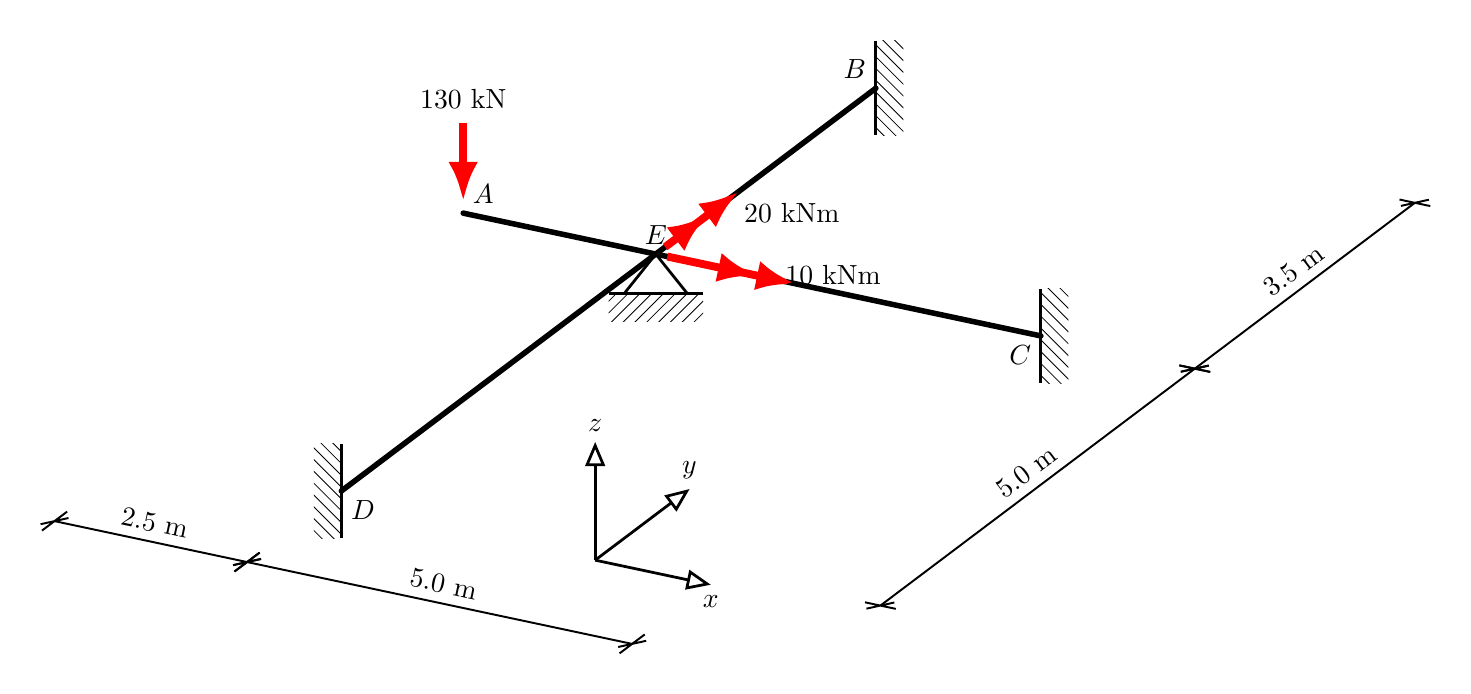
\begin{tikzpicture}[coords, background rectangle/.style={fill=white!46}, show background rectangle]

    \dpoint{a}{-2.5}{0}{0};
    \dpoint{e}{0}{0}{0}; 
    \dpoint{b}{0}{ 3.5 }{0}; 
    \dpoint{c}{ 5.0 }{0}{0};
    \dpoint{d}{0}{-5.0 }{0}; 
    \dpoint{z}{ 0.7*5.0 }{ -1.05*5.0 }{0}; 

    \daxis{1}{z}; 

    \foreach \startn/\endn in {e/a,e/b,e/c,e/d}
        \dbeam{1}{\startn}{\endn};

    \support{4ooo}{a}[270];
    \support{3}{b}[90];
    \support{3}{c}[90];
    \support{1}{e};
    \support{3}{d}[270];

    \begin{scope}[force/.append style={color=red,>={Latex[length=0pt 5]}},
    normalLine/.append style={line width=1mm}]
        \dload{1}{a}[0][90];
        \dnotation{1}{a}{$130$~kN}[above=12mm];
        
        \dload{4}{e}[90][90][ 3.5/3 ];
        \node[right=3mm] at ($(e)!0.25!(b)$) {$20$~kNm};

        \dload{4}{e}[90][0][ 5.0/3 ];
        %\dnotation{1}{e}{$!{n(Mx)}$~kNm}[below right=7mm];
        \node[right=3mm] at ($(e)!0.25!(c)$) {$10$~kNm};
    \end{scope}

    \ddimensioning{yx}{b}{e}{1.4*5.0}[$3.5$~m];
    \ddimensioning{yx}{e}{d}{1.4*5.0}[$5.0$~m];
    \ddimensioning{xy}{a}{e}{-1.3*5.0}[$2.5$~m];
    \ddimensioning{xy}{e}{c}{-1.3*5.0}[$5.0$~m];

    \dnotation{1}{e}{$E$}[above];
    \dnotation{1}{a}{$A$}[above right];
    \dnotation{1}{b}{$B$}[above left];
    \dnotation{1}{c}{$C$}[below left];
    \dnotation{1}{d}{$D$}[below right];

\end{tikzpicture}
        
\end{document}
